\documentclass[a4paper,12pt]{beamer}

\usepackage{préambule}
\usetikzlibrary{angles,arrows,arrows.meta,calc,intersections,quotes}

\begin{document}

\begin{frame}
	\begin{center}
		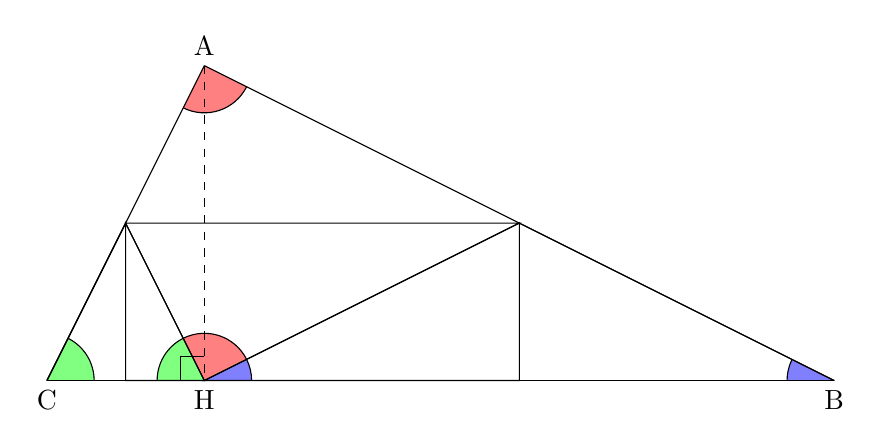
\begin{tikzpicture}
			\coordinate (A) at (2,4);
			\coordinate (B) at (10,0);
			\coordinate (C) at (0,0);
			\coordinate (H) at (2,0);

			\coordinate (D) at (1,2);
			\coordinate (E) at (6,2);
			\coordinate (F) at (6,0);
			\coordinate (G) at (1,0);

			\draw<3> pic[draw,fill=red!50,angle radius=0.6cm] {angle=C--A--B};
			\draw<4-> pic[draw,fill=red!50,angle radius=0.6cm] {angle=E--H--D};
			\draw<3-4> pic[draw,fill=blue!50,angle radius=0.6cm] {angle=A--B--C};
			\draw<5-> pic[draw,fill=blue!50,angle radius=0.6cm] {angle=F--H--E};
			\draw<3-5> pic[draw,fill=green!50,angle radius=0.6cm] {angle=B--C--A};
			\draw<6-> pic[draw,fill=green!50,angle radius=0.6cm] {angle=D--H--G};

			\draw<-3> (A) -- (B);
			\draw<4> (B) -- (E);
			\draw<4> (C) -- (D);
			\draw<-4> (B) -- (C);
			\draw<5> (C) -- (H);
			\draw<5> (C) -- (D);
			\draw<-3> (C) -- (A);

			\node<-3>[above] at (A) {A};
			\node<-4>[below] at (B) {B};
			\node<-5>[below] at (C) {C};

			\node<2->[below] at (H) {H};
			\draw<2-3>[dashed] (A) -- (H);
			\draw<2> (H) ++(-0.3,0) -- ++(0,0.3) -- ++(0.3,0);

			\draw<4-> (H) -- (D) -- (E) -- cycle;
			\draw<5-> (H) -- (E) -- (F) -- cycle;
			\draw<6-> (H) -- (D) -- (G) -- cycle;
		\end{tikzpicture}
	\end{center}
\end{frame}


\end{document}